% Appendix B — Figures

\chapter{Figures}

\label{app:figures}

All figures referenced in the main text are gathered here.

% ─────────────────────────────────────────────────────────────────────────────
\section*{B.1 --- Context \& Background}
% ─────────────────────────────────────────────────────────────────────────────

\begin{figure}[H]
    \centering
    \begin{subfigure}[t]{0.58\linewidth}
        \centering
        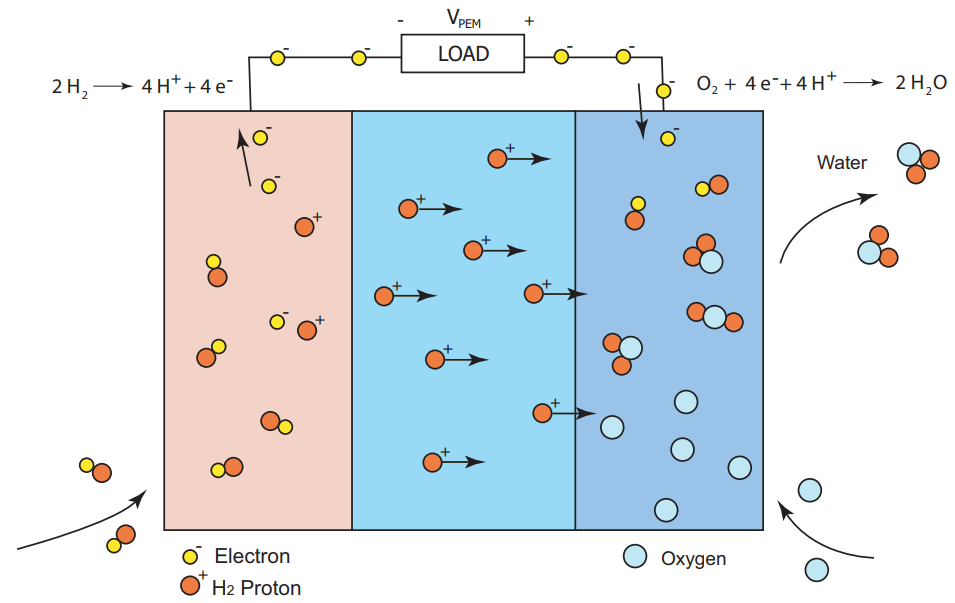
\includegraphics[width=\linewidth]{Figures/pemfc_operation.png}
        \caption{Basic electrochemical operation \cite{mohiuddin2018,thomya2011}.}
    \end{subfigure}
    \hfill
    \begin{subfigure}[t]{0.36\linewidth}
        \centering
        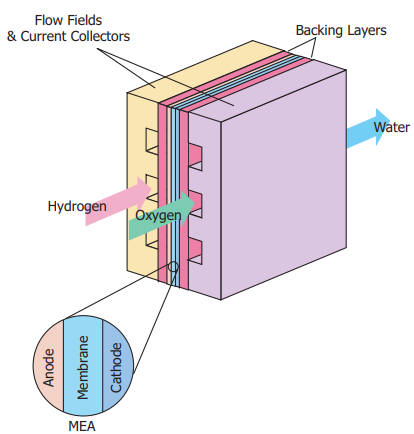
\includegraphics[width=\linewidth]{Figures/pemfc_stack_structure.png}
        \caption{Simplified stack structure and MEA \cite{manana2006}.}
    \end{subfigure}
    \caption{Operating principle and physical structure of a PEM fuel cell.}
    \label{fig:pemfc-operation}
\end{figure}

\begin{figure}[H]
    \centering
    \begin{subfigure}[t]{0.48\linewidth}
        \centering
        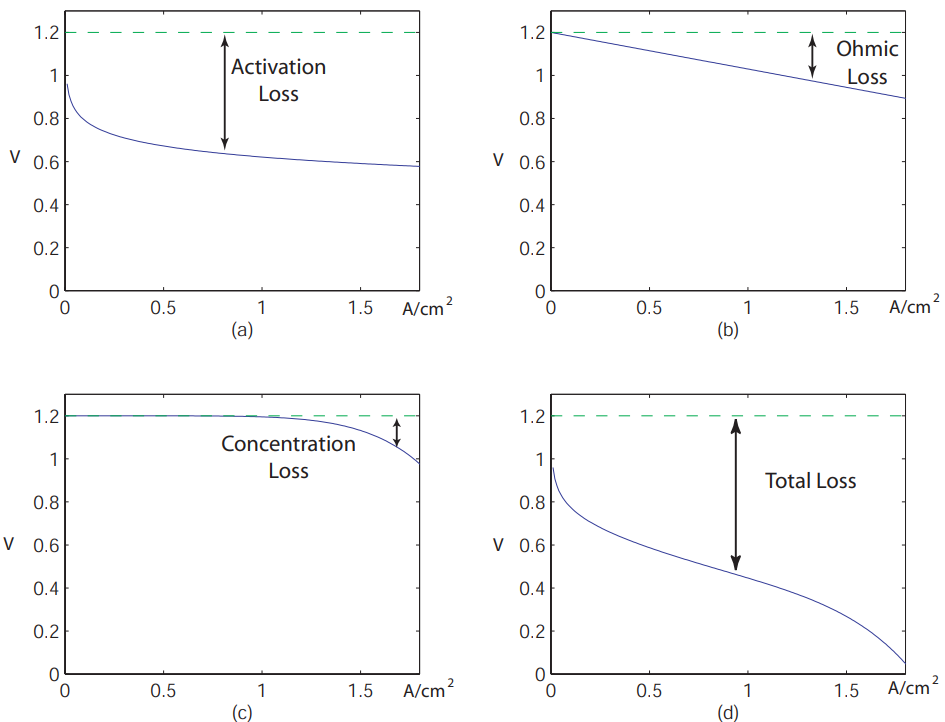
\includegraphics[width=\linewidth]{Figures/pemfc_loss_components.png}
        \caption{Activation, ohmic, concentration, and total losses.}
    \end{subfigure}
    \hfill
    \begin{subfigure}[t]{0.48\linewidth}
        \centering
        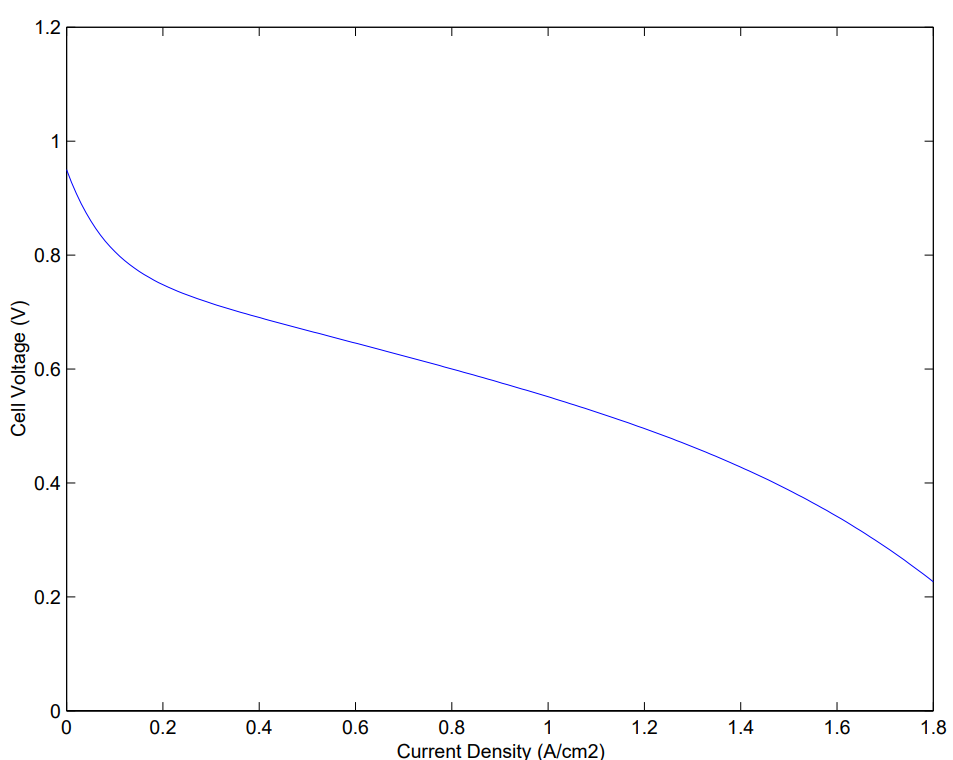
\includegraphics[width=\linewidth]{Figures/pemfc_polarization_curve.png}
        \caption{Typical polarization curve.}
    \end{subfigure}
    \caption{Influence of the main voltage losses on PEMFC performance.}
    \label{fig:pemfc-losses}
\end{figure}

% ─────────────────────────────────────────────────────────────────────────────
\section*{B.2 --- Model Architecture}
% ─────────────────────────────────────────────────────────────────────────────

\begin{figure}[H]
\centering
\resizebox{0.95\linewidth}{!}{%
\begin{tikzpicture}[
    >=Latex,
    block/.style={draw, rectangle, thick, fill=white, align=center,
        text width=4.5cm, minimum height=1.9cm, inner sep=6pt, font=\small},
    vblock/.style={draw, rectangle, thick, fill=white, align=center,
        text width=5.4cm, minimum height=1.85cm, inner sep=6pt, font=\small},
    oblock/.style={draw, rectangle, thick, fill=white, align=center,
        text width=4.8cm, minimum height=1.6cm, inner sep=6pt, font=\small},
    lab/.style={font=\scriptsize, align=center},
    line/.style={-{Latex[length=2mm,width=1.4mm]}, line width=0.8pt}
]
\node[block] (anode) {\textbf{Anode subsystem}\\[0.15em]
Hydrogen mass balance\\ Water balance\\ Outputs: $P_{H_2},\,\phi_{an}$};
\node[block, right=2.8cm of anode] (membrane) {\textbf{Membrane subsystem}\\[0.15em]
Hydration / water transport\\ Electro-osmotic drag\\ Back-diffusion\\ Output: $W_{v,mbr}$};
\node[block, right=2.8cm of membrane] (cathode) {\textbf{Cathode subsystem}\\[0.15em]
Constant $P_{O_2}^{\ast}=0.21P_{\mathrm{atm}}$\\ Water balance + reaction water\\ Output: $\phi_{ca}$};
\node[vblock, below=1.50cm of membrane] (voltage) {\textbf{Fuel cell voltage block}\\[0.15em]
$E-v_{act}-v_{ohm}-v_{con}$\\ Inputs: $P_{H_2},\,P_{O_2}^{\ast},\,i_{FC},\,T,$ membrane state};
\node[oblock, below=1.0cm of voltage] (output) {\textbf{Model outputs}\\[0.15em]
Cell voltage and internal states\\ ($P_{H_2},\,\phi_{an},\,\phi_{ca},\,W_{v,mbr}$)};
\node[lab, above=0.2cm of anode] {$W_{H_2,in},\,i_{FC},\,T$};
\node[lab, above=0.2cm of membrane] {$i_{FC},\,T,\,\phi_{an},\,\phi_{ca}$};
\node[lab, above=0.2cm of cathode] {$i_{FC},\,T$};
\draw[line] ([yshift=5pt]anode.east) -- node[above,lab] {$\phi_{an}$} ([yshift=5pt]membrane.west);
\draw[line] ([yshift=-7pt]membrane.west) to[bend right=18]
    node[below,lab] {$W_{v,mbr}$} ([yshift=-7pt]anode.east);
\draw[line] ([yshift=5pt]cathode.west) -- node[above,lab] {$\phi_{ca}$} ([yshift=5pt]membrane.east);
\draw[line] ([yshift=-7pt]cathode.west) to[bend right=18]
    node[below,lab] {$W_{v,mbr}$} ([yshift=-7pt]membrane.east);
\draw[line] (anode.south) |- node[pos=0.23,left,lab] {$P_{H_2}$} (voltage.west);
\draw[line] (membrane.south) -- node[right,lab] {membrane\\state} (voltage.north);
\node[lab, right=0.95cm of voltage] {$P_{O_2}^{\ast}=0.21P_{\mathrm{atm}}$};
\draw[line] (voltage.south) -- (output.north);
\end{tikzpicture}%
}
\caption{Block-level architecture of the reduced PEMFC model.}
\label{fig:architecture}
\end{figure}

% ─────────────────────────────────────────────────────────────────────────────
\section*{B.3 --- Parameter Identification, Optimization Experiment}
% ─────────────────────────────────────────────────────────────────────────────

\begin{figure}[H]
    \centering
    
\includegraphics[width=0.88\linewidth]{Figures/cost_evolution_exp19.png}
    \caption{DE optimizer convergence history for all ten cells --- Optimization
             Experiment. Dashed line: final RMSE after L-BFGS-B refinement.}
    \label{fig:cost-evolution}
\end{figure}

\begin{figure}[H]
    \centering
    
\includegraphics[width=\linewidth]{Figures/all_cells_overview_exp19.png}
    \caption{Per-cell $V$--$I$ calibration fits --- Optimization Experiment.}
    \label{fig:vi-opt}
\end{figure}

\begin{figure}[H]
    \centering
    
\includegraphics[width=\linewidth]{Figures/comparison_exp19_cells.png}
    \caption{Per-cell voltage, measured vs.\ simulated --- Optimization
             Experiment. Cells~0, 1, 2 collapse under load (hardware
             degradation). Mean RMSE (healthy cells) = 8.0\,mV.}
    \label{fig:ts-opt-cells}
\end{figure}

\begin{figure}[H]
    \centering
    
\includegraphics[width=0.85\linewidth]{Figures/comparison_exp19_stack.png}
    \caption{Stack voltage, load current and hydrogen pressure --- Optimization
             Experiment. Load applied at $t=135$\,s, removed at $t=684$\,s.}
    \label{fig:ts-opt-stack}
\end{figure}

\begin{figure}[H]
    \centering
    
\includegraphics[width=0.85\linewidth]{Figures/comparison_exp19_error.png}
    \caption{Per-cell voltage error (simulated $-$ measured) --- Optimization
             Experiment.}
    \label{fig:ts-opt-error}
\end{figure}

% ─────────────────────────────────────────────────────────────────────────────
\section*{B.4 --- TR-Current Step-Response Experiments}
% ─────────────────────────────────────────────────────────────────────────────

\begin{figure}[H]
    \centering
    \begin{subfigure}[t]{0.49\linewidth}
        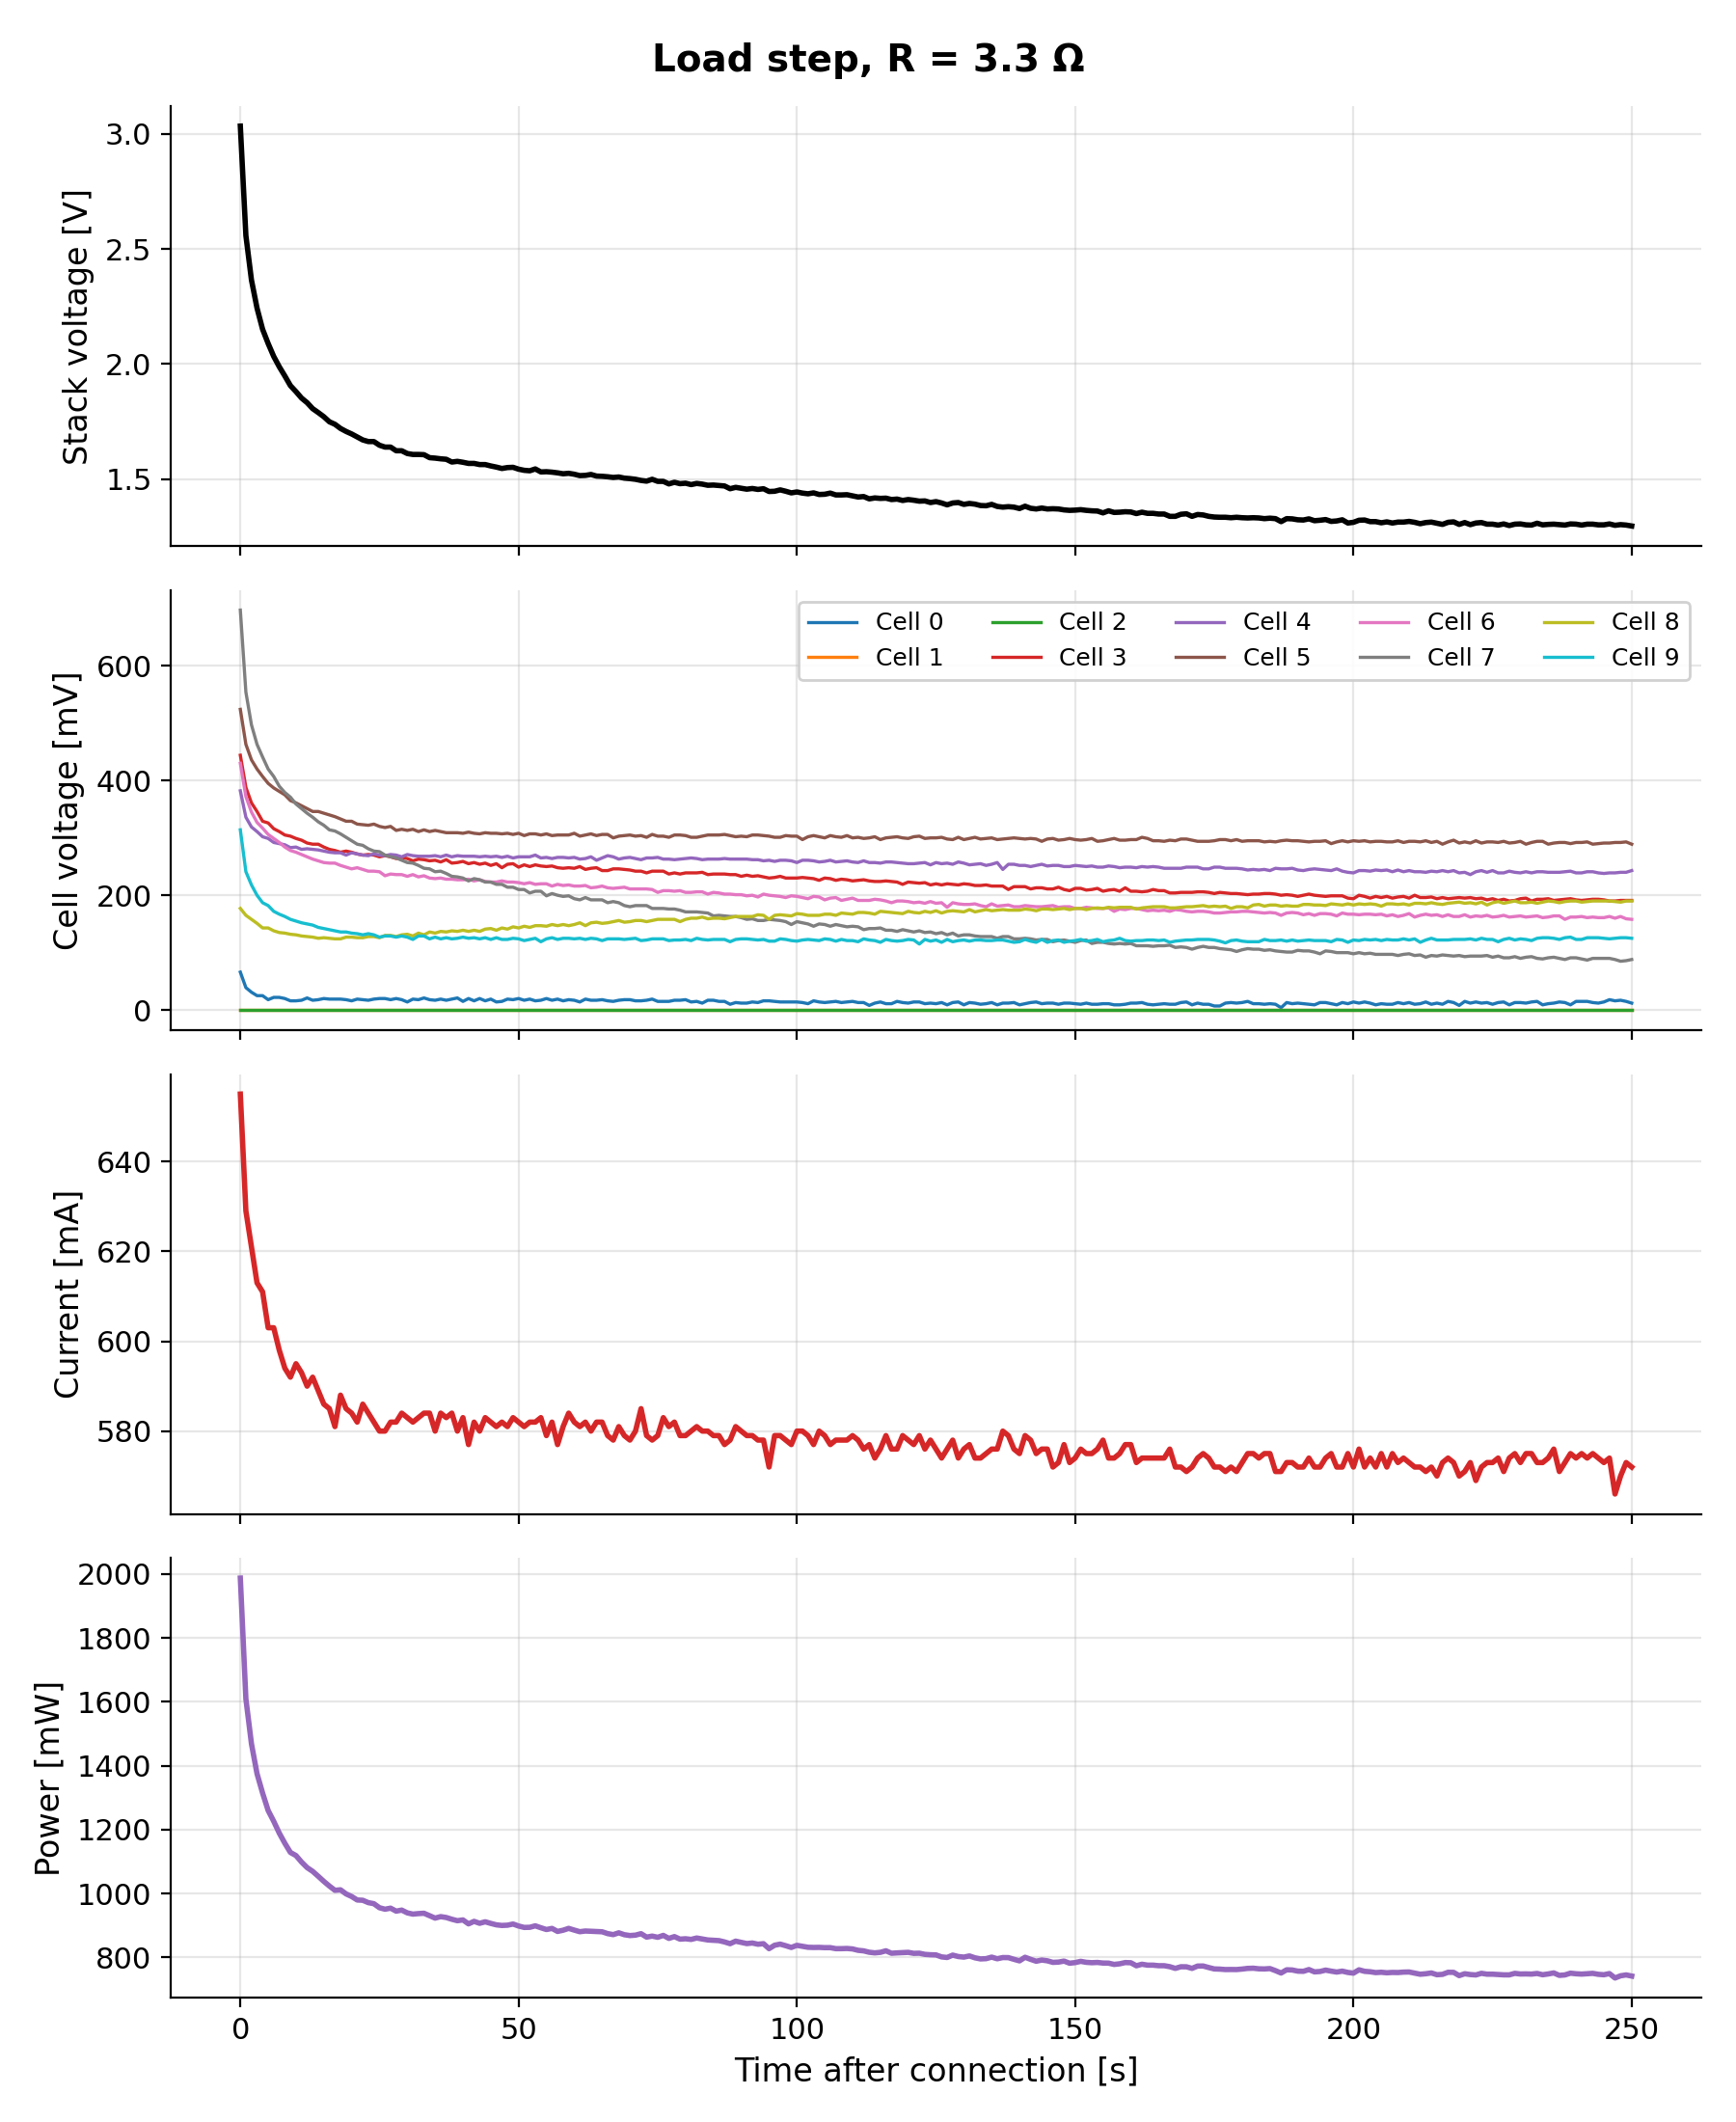
\includegraphics[width=\linewidth]{Figures/exp_33ohm_plot.png}
        \caption{Experiment~1 ($R=3.3\,\Omega$, 0--250\,s).}
    \end{subfigure}\hfill
    \begin{subfigure}[t]{0.49\linewidth}
        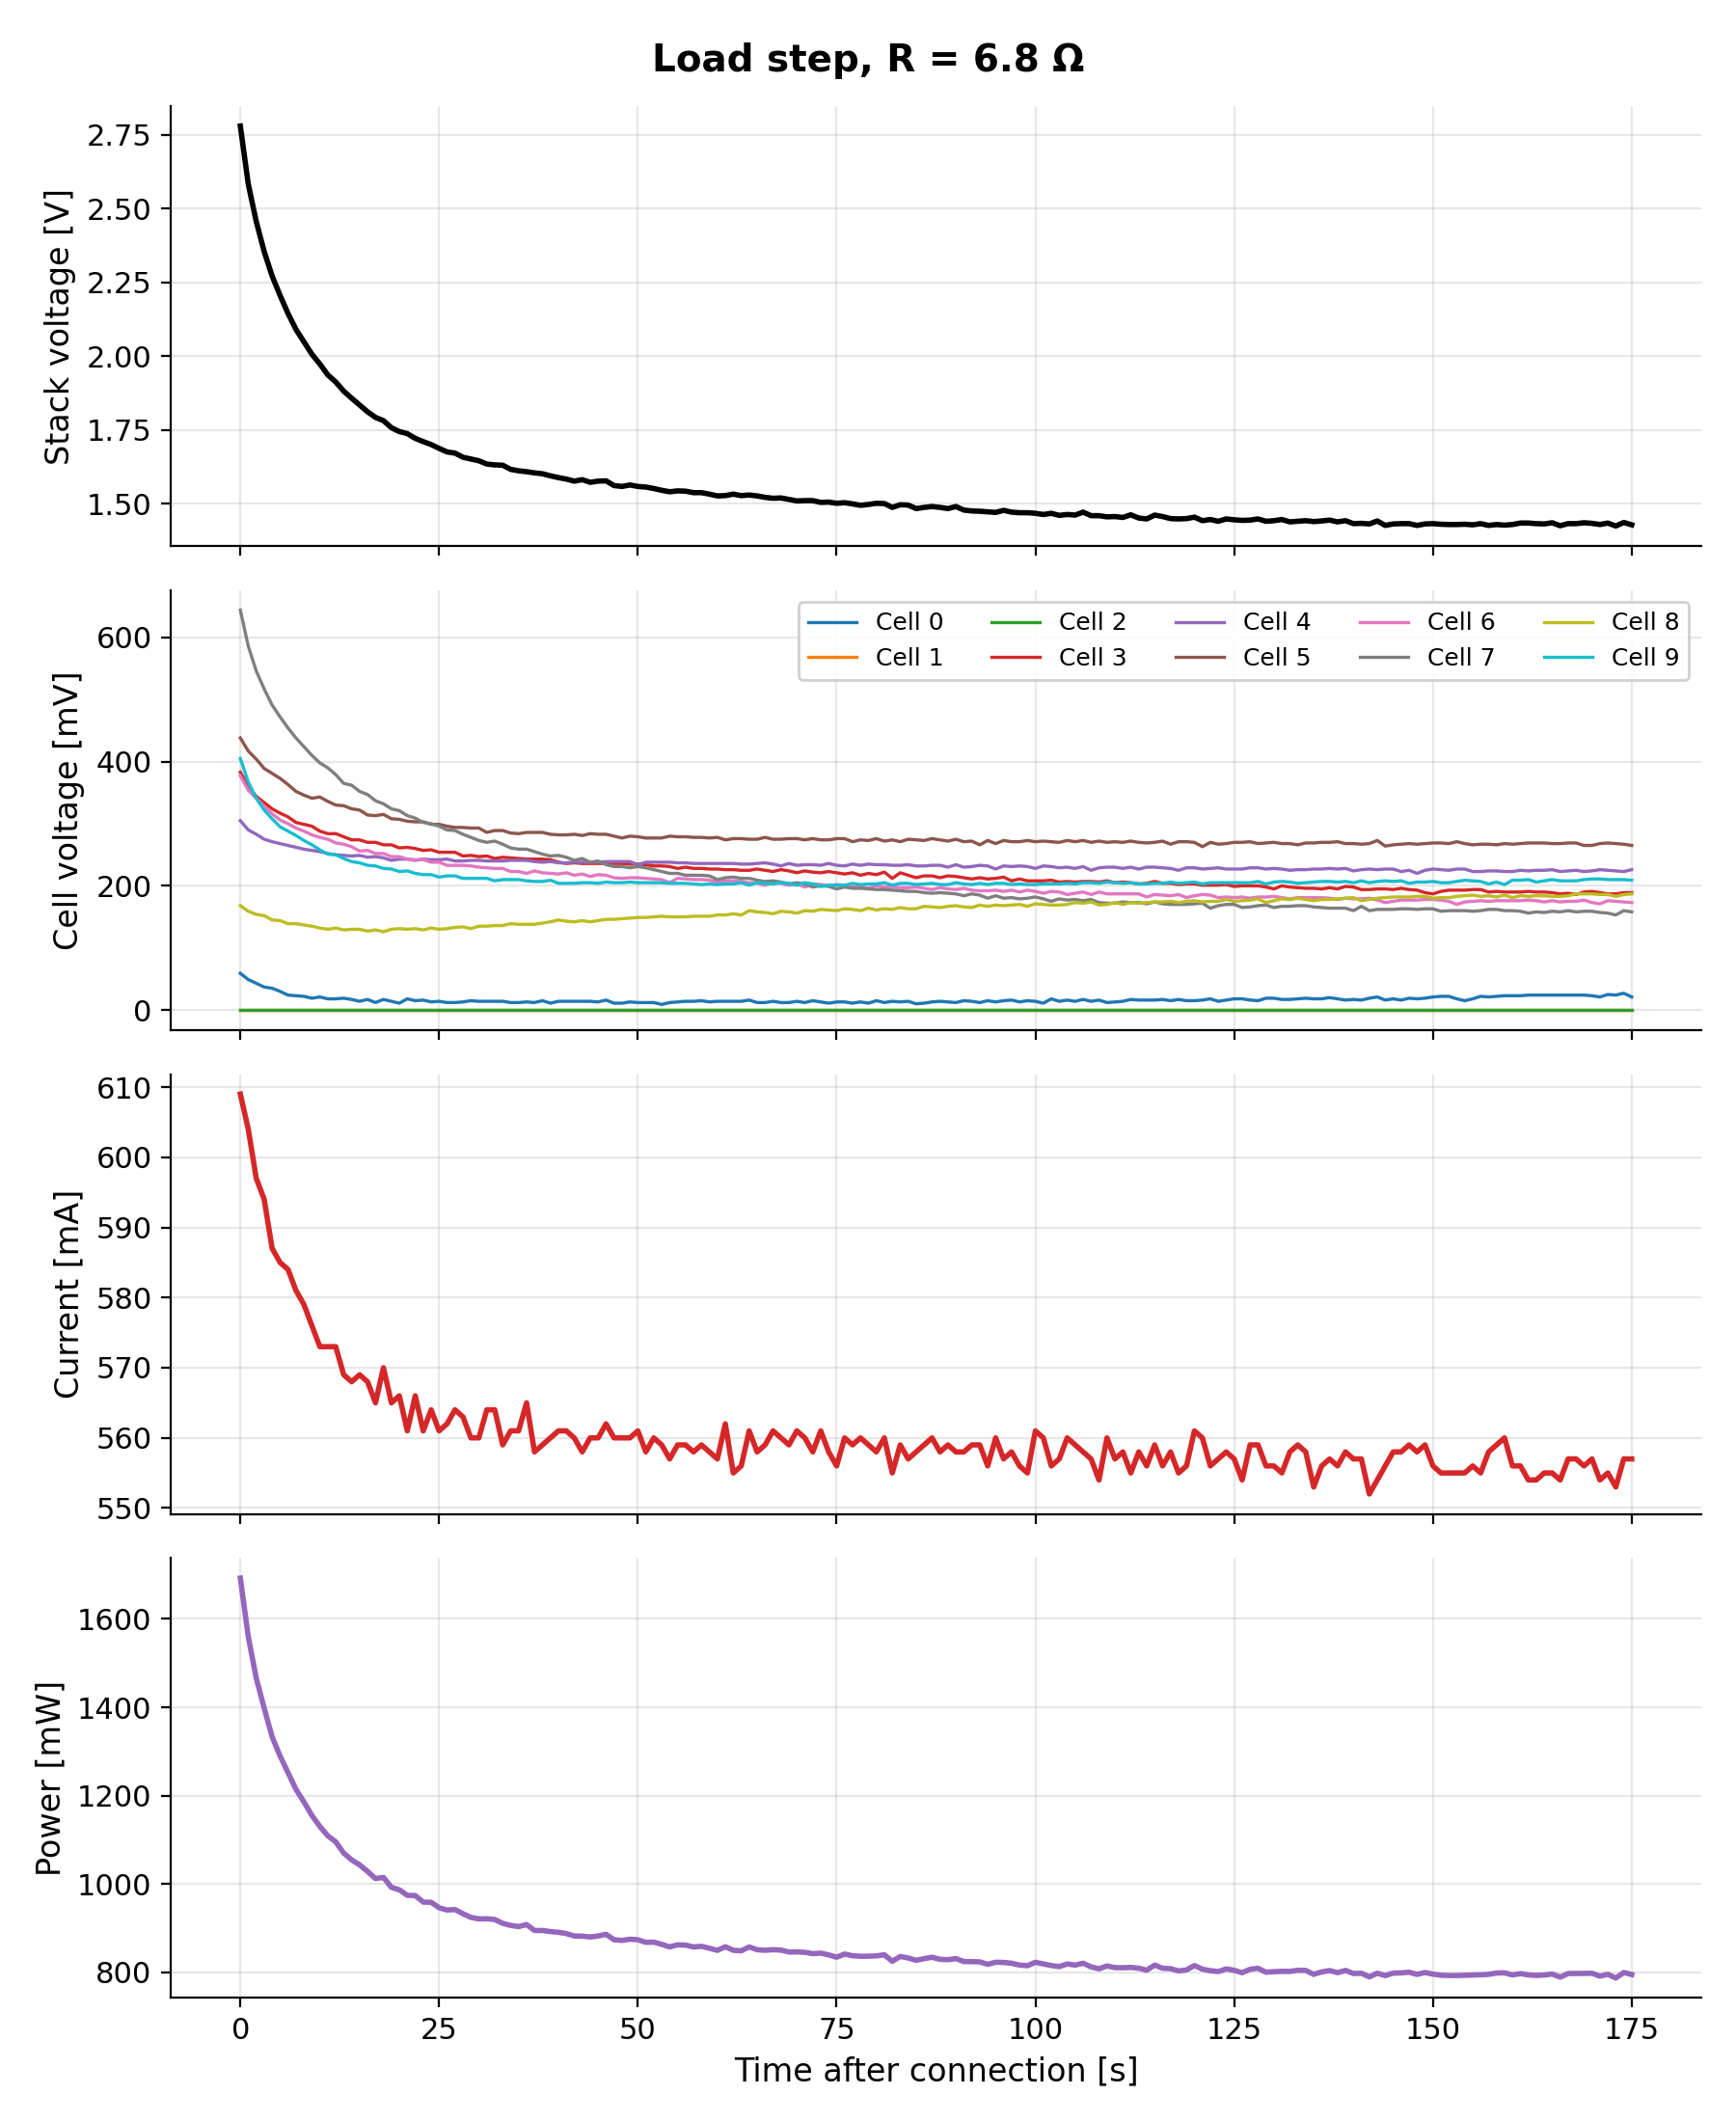
\includegraphics[width=\linewidth]{Figures/exp_68ohm_plot.png}
        \caption{Experiment~4 ($R=6.8\,\Omega$, 0--175\,s).}
    \end{subfigure}
    \caption{TR-current experiments: stack voltage [V], cell voltages [mV],
             current [mA], and power $P=V_{\text{stack}}\cdot I$ [mW].}
    \label{fig:tr-experiments}
\end{figure}

\begin{figure}[H]
    \centering
    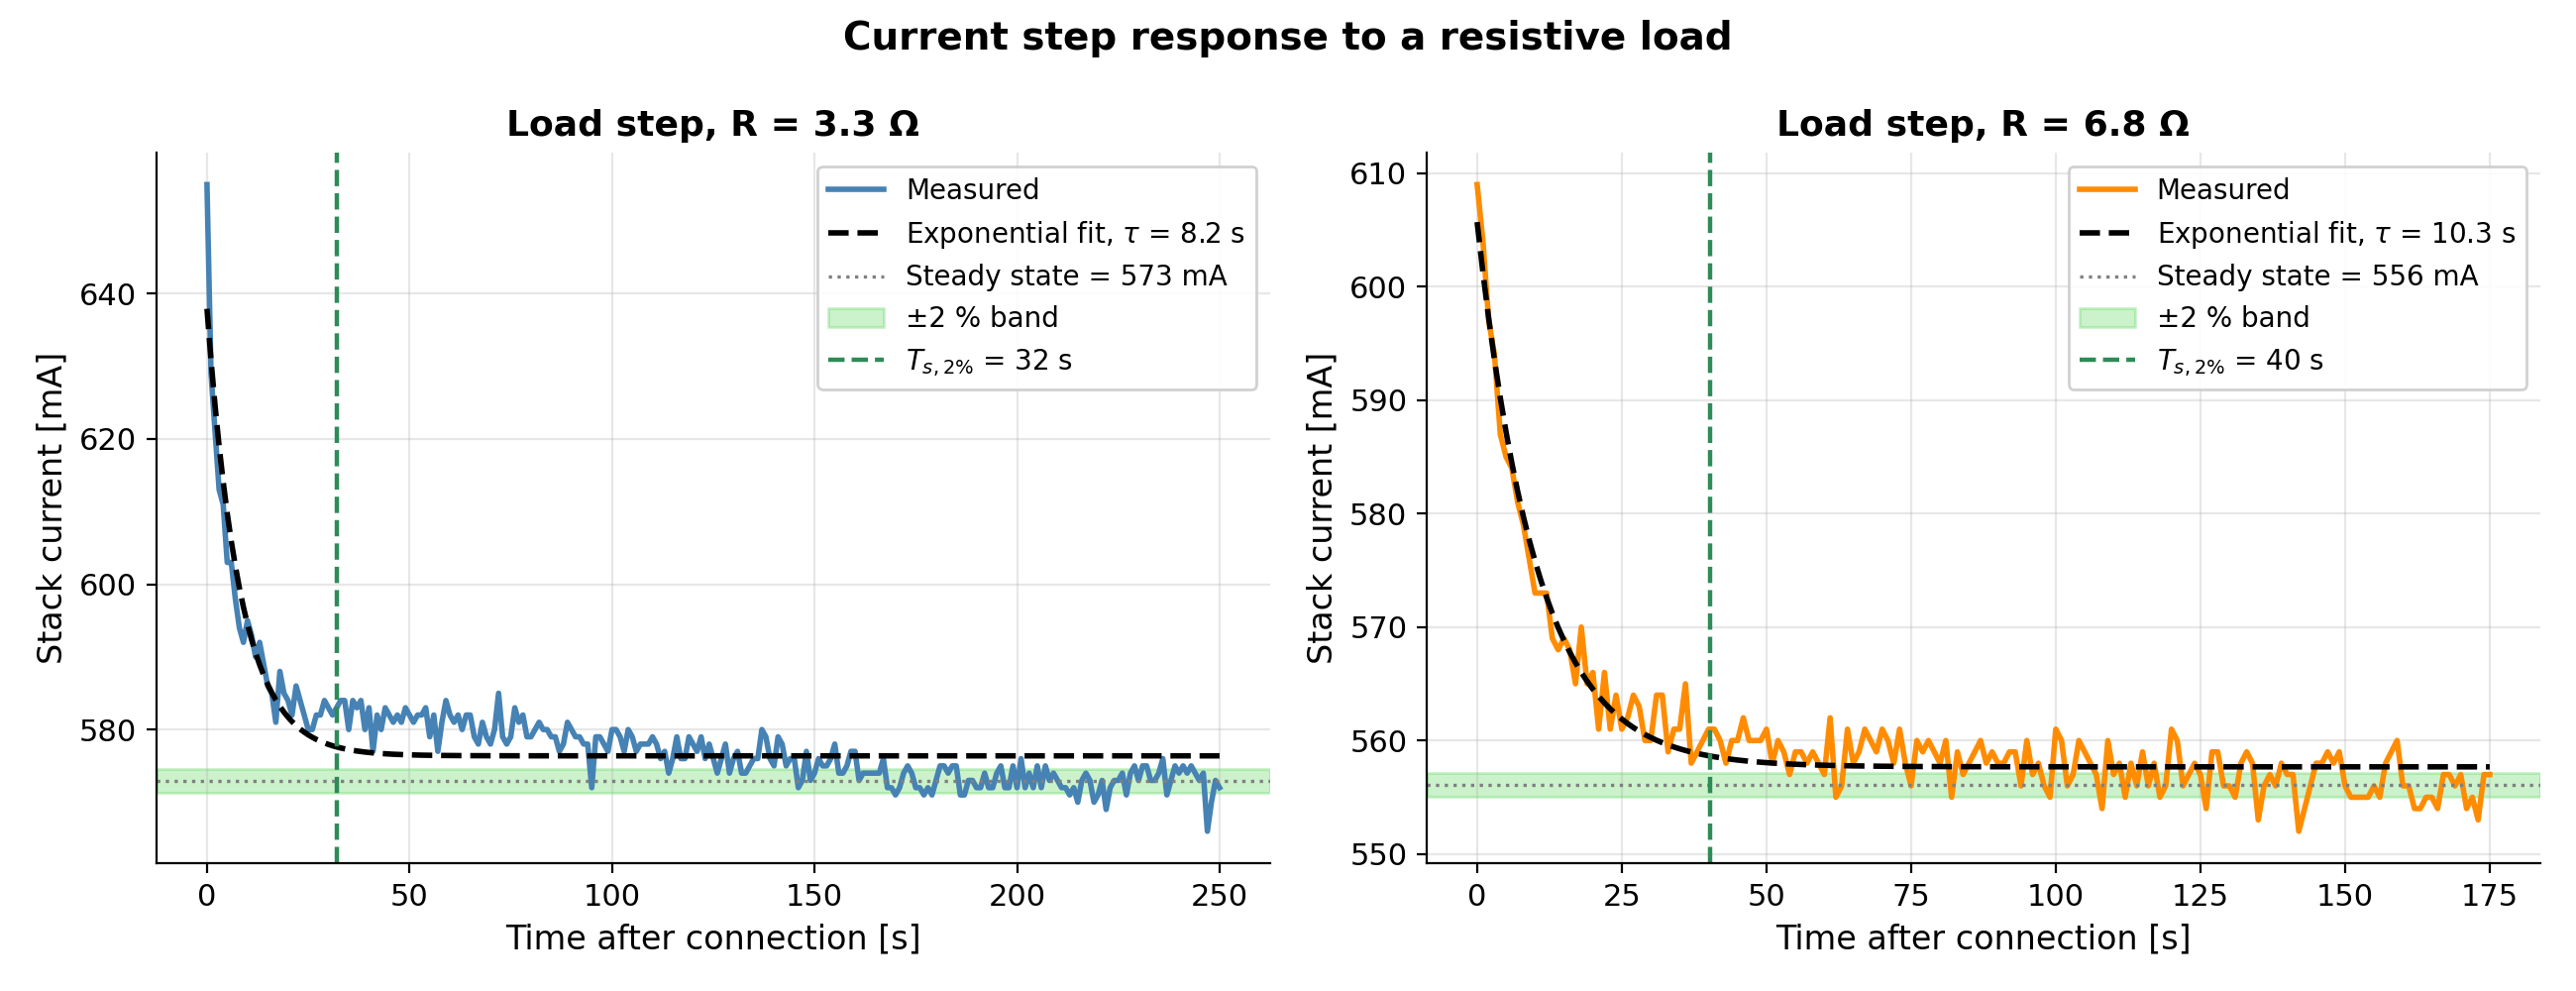
\includegraphics[width=0.72\linewidth]{Figures/response_time_plot.png}
    \caption{Current step response after resistor connection: measured data
             (color), exponential fit (dashed), steady-state band, and
             settling-time markers.}
    \label{fig:tr-responses}
\end{figure}

% ─────────────────────────────────────────────────────────────────────────────
\section*{B.5 --- Control Architecture}
% ─────────────────────────────────────────────────────────────────────────────

\begin{figure}[H]
\centering
\begin{tikzpicture}[
    >=Latex,
    blk/.style={draw, rectangle, thick, fill=white, align=center,
        minimum height=1.3cm, minimum width=2.6cm, inner sep=5pt, font=\small},
    sums/.style={draw, circle, thick, minimum size=0.55cm, inner sep=0pt},
    lab/.style={font=\scriptsize, align=center},
    line/.style={-{Latex[length=2mm,width=1.4mm]}, line width=0.8pt}
]
\node[blk] (fc) {\textbf{PEMFC stack}\\ (current or\\ voltage source)};
\node[blk, right=1.7cm of fc] (boost) {\textbf{DC/DC boost}\\ \textbf{converter}};
\node[blk, right=1.7cm of boost] (load) {\textbf{Load}};
\node[blk, below=1.4cm of boost] (pwm) {\textbf{PWM}};
\node[blk, left=1.5cm of pwm] (pi) {\textbf{PI controller}\\ $u=K_P e + K_I\!\int\! e\,dt$};
\node[sums, left=1.3cm of pi] (sumj) {};
\node[lab, above left=1pt and 1pt of sumj.north west] {$+$};
\node[lab, below right=4pt and -2pt of sumj.south] {$-$};

\draw[line] (fc) -- node[above,lab] {$V_{STACK}$} (boost);
\draw[line] (boost) -- node[above,lab] {$V_{OUT}$} (load);
\draw[line] (pwm) -- node[right,lab] {duty cycle $T$} (boost);
\draw[line] (pi) -- (pwm);
\draw[line] (sumj) -- node[above,lab] {$e$} (pi);
\draw[line] ([xshift=-1.1cm]sumj.west) -- node[above,lab] {$I_{REF}$ (or $V_{REF}$)} (sumj);
\draw[line] ([xshift=0.55cm]boost.south) |- ([yshift=-1.05cm]pi.south)
    -| node[pos=0.25,below,lab] {measured $I_L$ (or $V_{OUT}$)} (sumj);
\end{tikzpicture}
\caption{Control architecture of the PEMFC power system, after
         \cite{derbeli2017}: the stack feeds a DC/DC boost converter whose duty
         cycle is set by a PI controller. Regulating the inductor current $I_L$
         makes the converter output behave as a current source; regulating the
         output voltage $V_{OUT}$ makes it behave as a voltage source.}
\label{fig:boost-architecture}
\end{figure}
